\section{Experimental results}

\subsection{Evaluation protocol and classification accuracy}
\label{sec:accuracy}
Peak validation checkpoints were monitored with~\texttt{scripts/train\_*.py}.
Unless stated otherwise, we report stratified pooling of \(\sim\)85\% training and \(\sim\)15\% withheld validation segments with identical random seed across models.
All subjects contribute to both partitions; therefore the protocol indexes pooled mixing across participants rather than the leave-one-subject-out evaluation advocated for clinical extrapolation~\cite{ofner2017upper}.

Table~\ref{tab:main} summarises withheld accuracy ranks.
CNN temporal encoding improves markedly relative to CSP (\(\approx +18\) percentage points), whereas PSD concatenation contributes roughly five additional points (\(\approx 56 \rightarrow 61\%\)).
Connectivity attention aligns with PSD fusion (\(\approx 61\mbox{--}62\%\)), indicating that multimodal augmentation alone does not reposition the optimisation landscape enough to transcend the EEGNet plateau---consistent with the hypothesis that temporal receptive fields disproportionately dominate learning dynamics.

\begin{table}[t]
  \centering
  \caption{Held-out multiclass accuracy (four coarse motor states vs.\ rest); chance\,=\,25\%.}
  \label{tab:main}
  \footnotesize
  \setlength{\tabcolsep}{3pt}
  \resizebox{\columnwidth}{!}{%
  \begin{tabular}{@{}llc@{}}
    \toprule
    \textbf{Architecture} & \textbf{Representations} & \textbf{Accuracy [\%]} \\
    \midrule
    CSP+LDA~\cite{gramfort2013meg} & CSP log-energy (six filters) & $\sim{}38^{\dagger}$ \\
    EEGNet~\cite{lawhern2018eegnet} & raw waveform convolution & $\sim{}56$ \\
    \texttt{EEGPsdNet} & waveform + Welch PSD~(late fuse) & $\sim{}61$ \\
    \texttt{EEGConnNet}$^{\ddagger}$ & waveform + Morlet CSD~(attention) & $\sim{}61\mbox{--}62$ \\
    \bottomrule
  \end{tabular}}
  \\[3pt]
  \raggedright\scriptsize
  $^{\dagger}$Higher CSP~(38.5\%) appears under narrow-band sweeps~\texttt{tune\_csp\_grid.json}; CSP on exported wide-band tensors can fall nearer 32\% (\texttt{csp\_lda.ipynb}).
  $^{\ddagger}$Implementation~\texttt{EEGConnectivityNet} in~\texttt{src/networks.py}.
\end{table}

\subsection{Connectivity topographies contrasting hand movement and rest}
\label{sec:topo}
Connectivity-derived contrasts between \emph{hand} synergy epochs and \emph{rest} reveal structured spatial modulation over motor-centred electrodes~\cite{ofner2017upper}: sensorimotor band coupling differentiates behavioural states despite limited downstream classifier separation.
Hence neurophysiological plausibility and statistical classification performance furnish complementary diagnoses---motor-network fingerprints can remain visible while discriminative variance for fine-grained multiclass boundaries lingers predominantly in nuisance-rich temporal residuals.

\begin{figure*}[t]
  \centering
  
\includegraphics[width=\linewidth]{connectivity_topomaps}
  \caption{Connectivity-based scalp maps contrasting hand-related movement epochs with resting baselines~(trial-averaged coupling summaries mapped to electrodes; Graz montage~\cite{ofner2017upper}). Contralateral and peri-central modulation indicates that coherence-inspired features encode task-relevant structure even though end-to-end accuracies saturate near the EEGNet PSD baseline.}
  \label{fig:connTopo}
\end{figure*}

\subsection{Latent geometry before softmax}

Penultimate embeddings were nonlinearly embedded with identical t-SNE hyper-parameters~(Figure~\ref{fig:tsne}).
Colours remain interleaved across EEGNet and both fusion architectures, confirming that softmax inputs occupy partially overlapping neighbourhoods.
Interpretation remains qualitative because t-SNE nonlinearly warps distances; nevertheless pervasive colour mixing parallels the accuracy plateau induced by multimodal fusion.

\begin{figure*}[t]
  \centering
  \begin{subfigure}[t]{0.32\textwidth}
    \centering
    
\includegraphics[width=\linewidth]{TSNE_EEGNet_Latent_Space_predecision}
    \caption{EEGNet}
    \label{fig:tsne-eegnet}
  \end{subfigure}\hfill
  \begin{subfigure}[t]{0.32\textwidth}
    \centering
    
\includegraphics[width=\linewidth]{TSNE_EEGPsdNet_Latent_Space_predecision}
    \caption{\texttt{EEGPsdNet}}
    \label{fig:tsne-psd}
  \end{subfigure}\hfill
  \begin{subfigure}[t]{0.32\textwidth}
    \centering
    
\includegraphics[width=\linewidth]{TSNE_EEGConnNet_Latent_Space_predecision}
    \caption{\texttt{EEGConnectivityNet}}
    \label{fig:tsne-conn}
  \end{subfigure}
  \caption{t-SNE visualisations of pre-softmax embeddings for withheld trials.}
  \label{fig:tsne}
\end{figure*}

\subsection{Confusion structure}
\label{sec:cf}
Diagonal concentration improves from CSP through CNN fusion, yet off-diagonal leakage persists predominantly among neighbouring synergies~(Figure~\ref{fig:cms}), echoing Figures~\ref{fig:connTopo}--\ref{fig:tsne}.
Training-validation divergence in archived learning curves~\texttt{models/*/learning\_curves.png} indicates that waveform branches reduce training losses faster while auxiliary branches saturate earlier.

\begin{figure}[t]
  \centering
  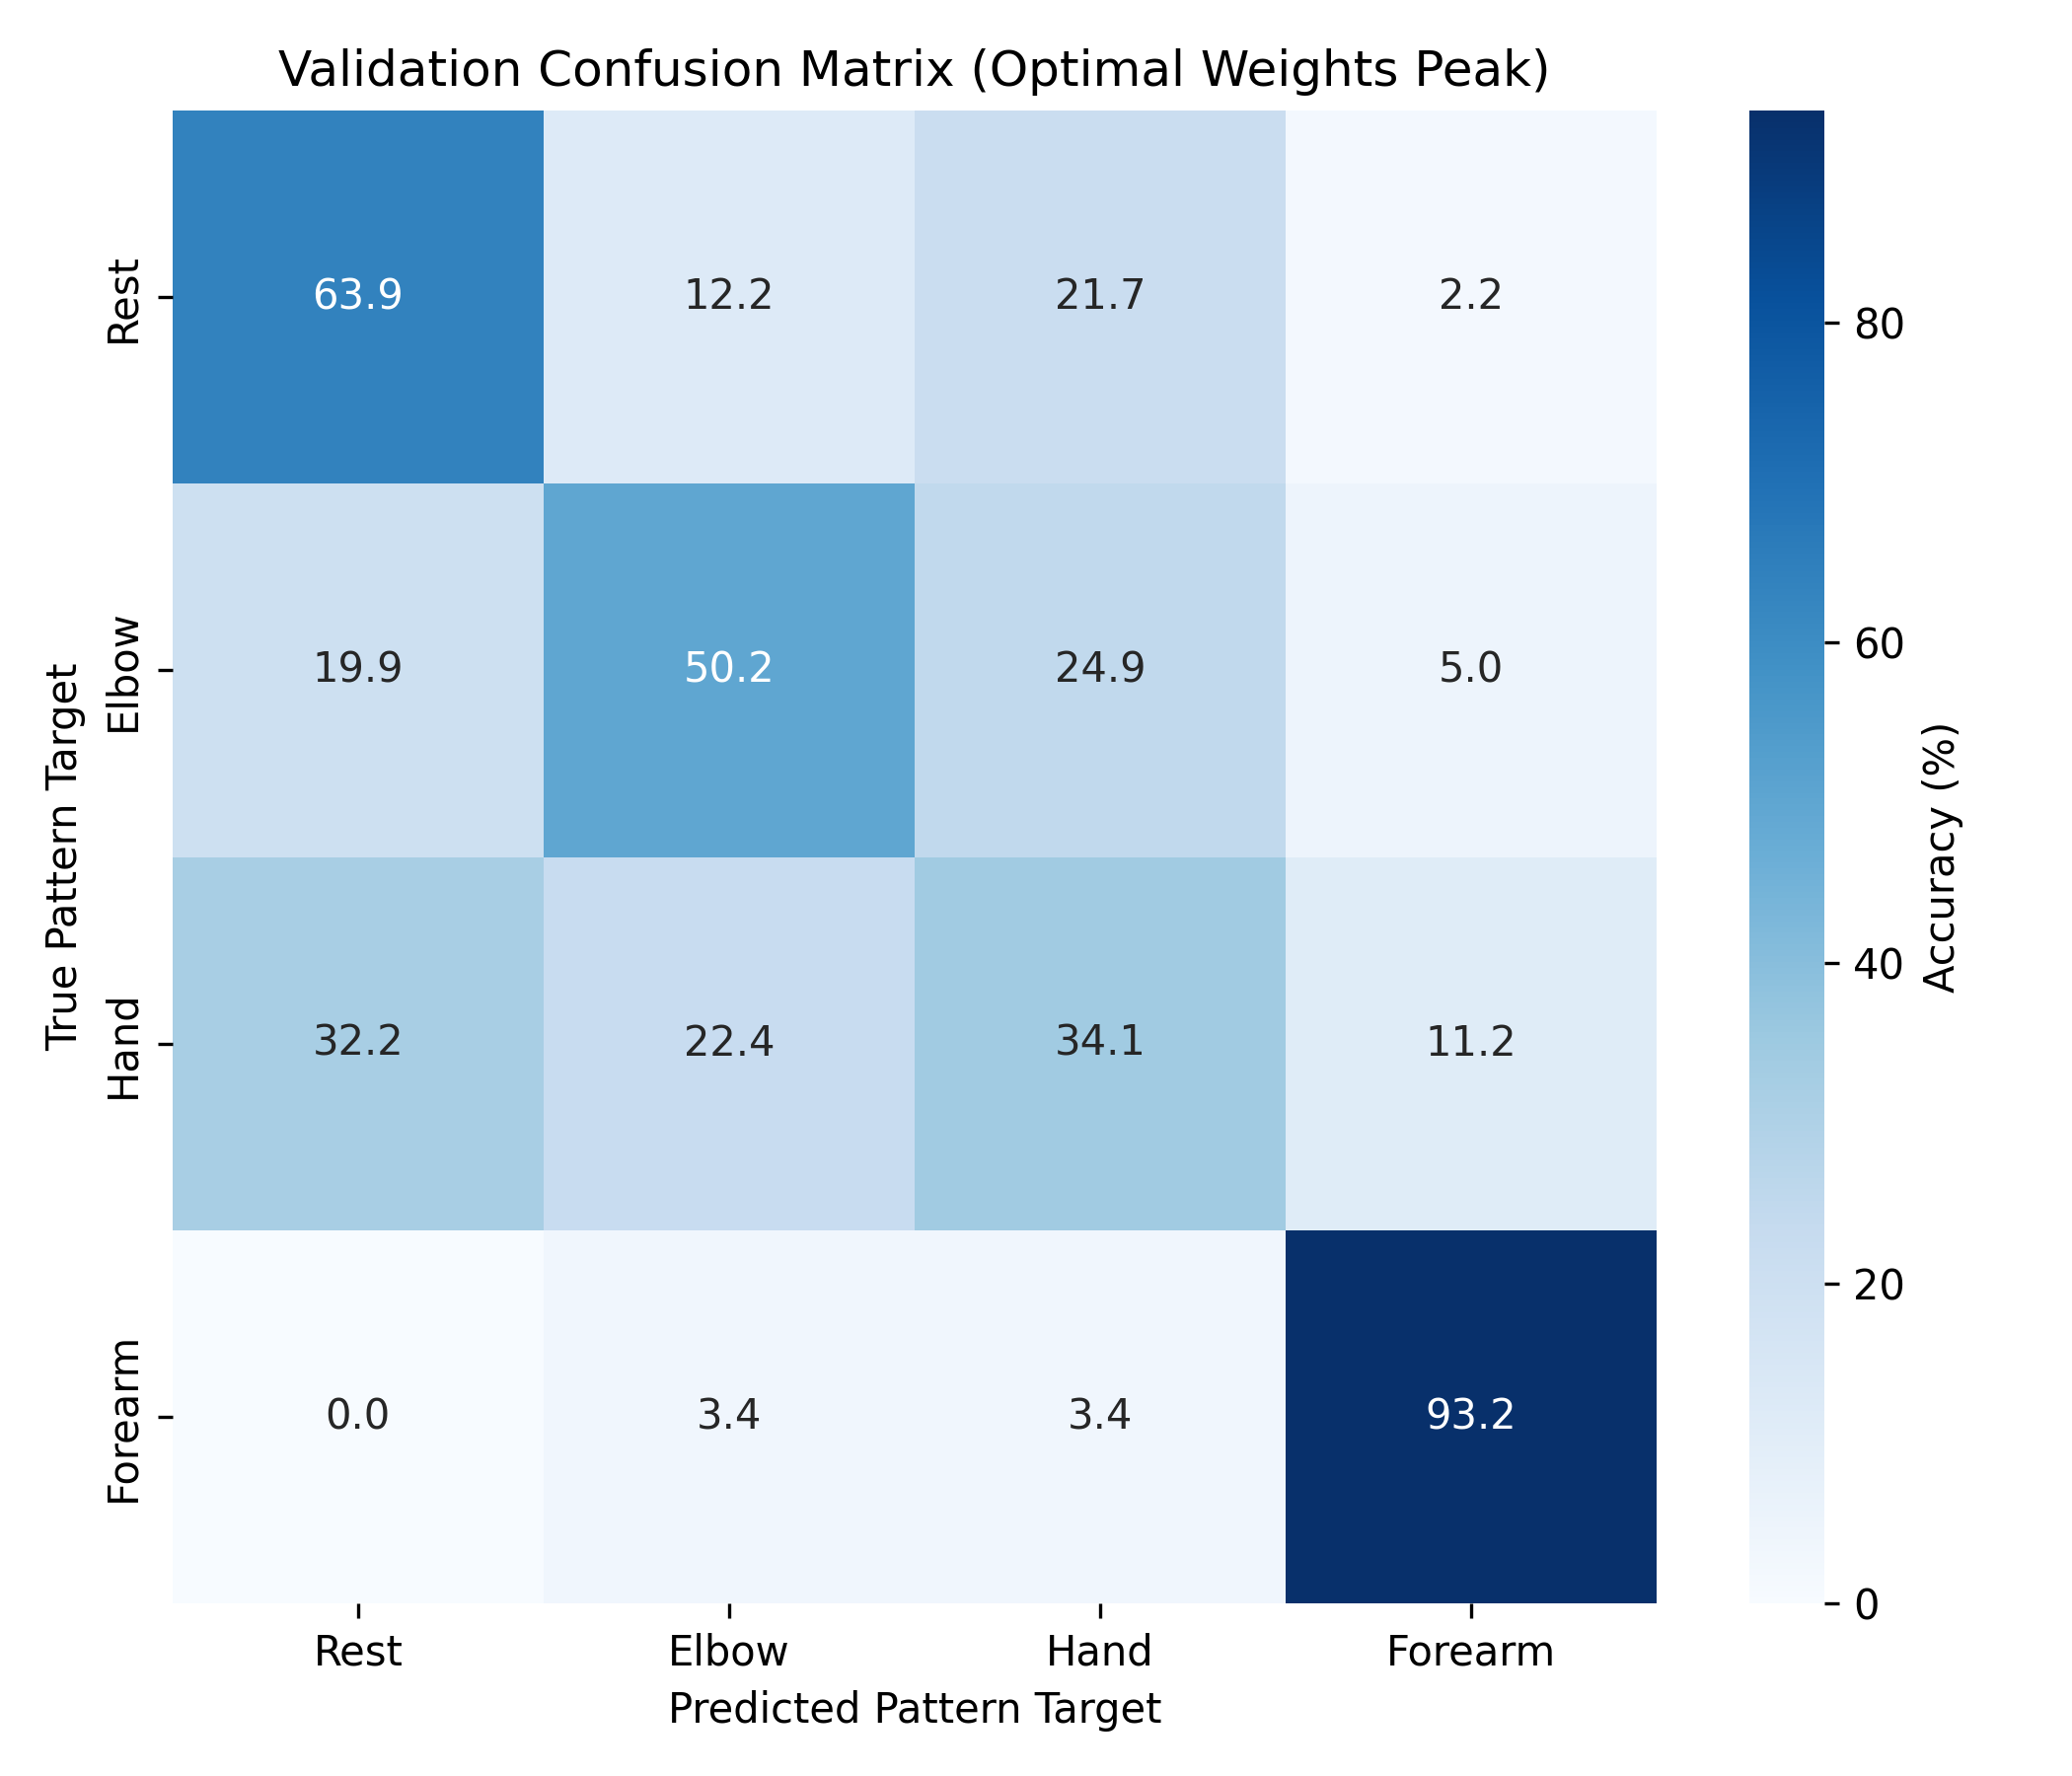
\includegraphics[width=0.324\linewidth]{models/eeg_net/confusion_matrix.png}\hfill
  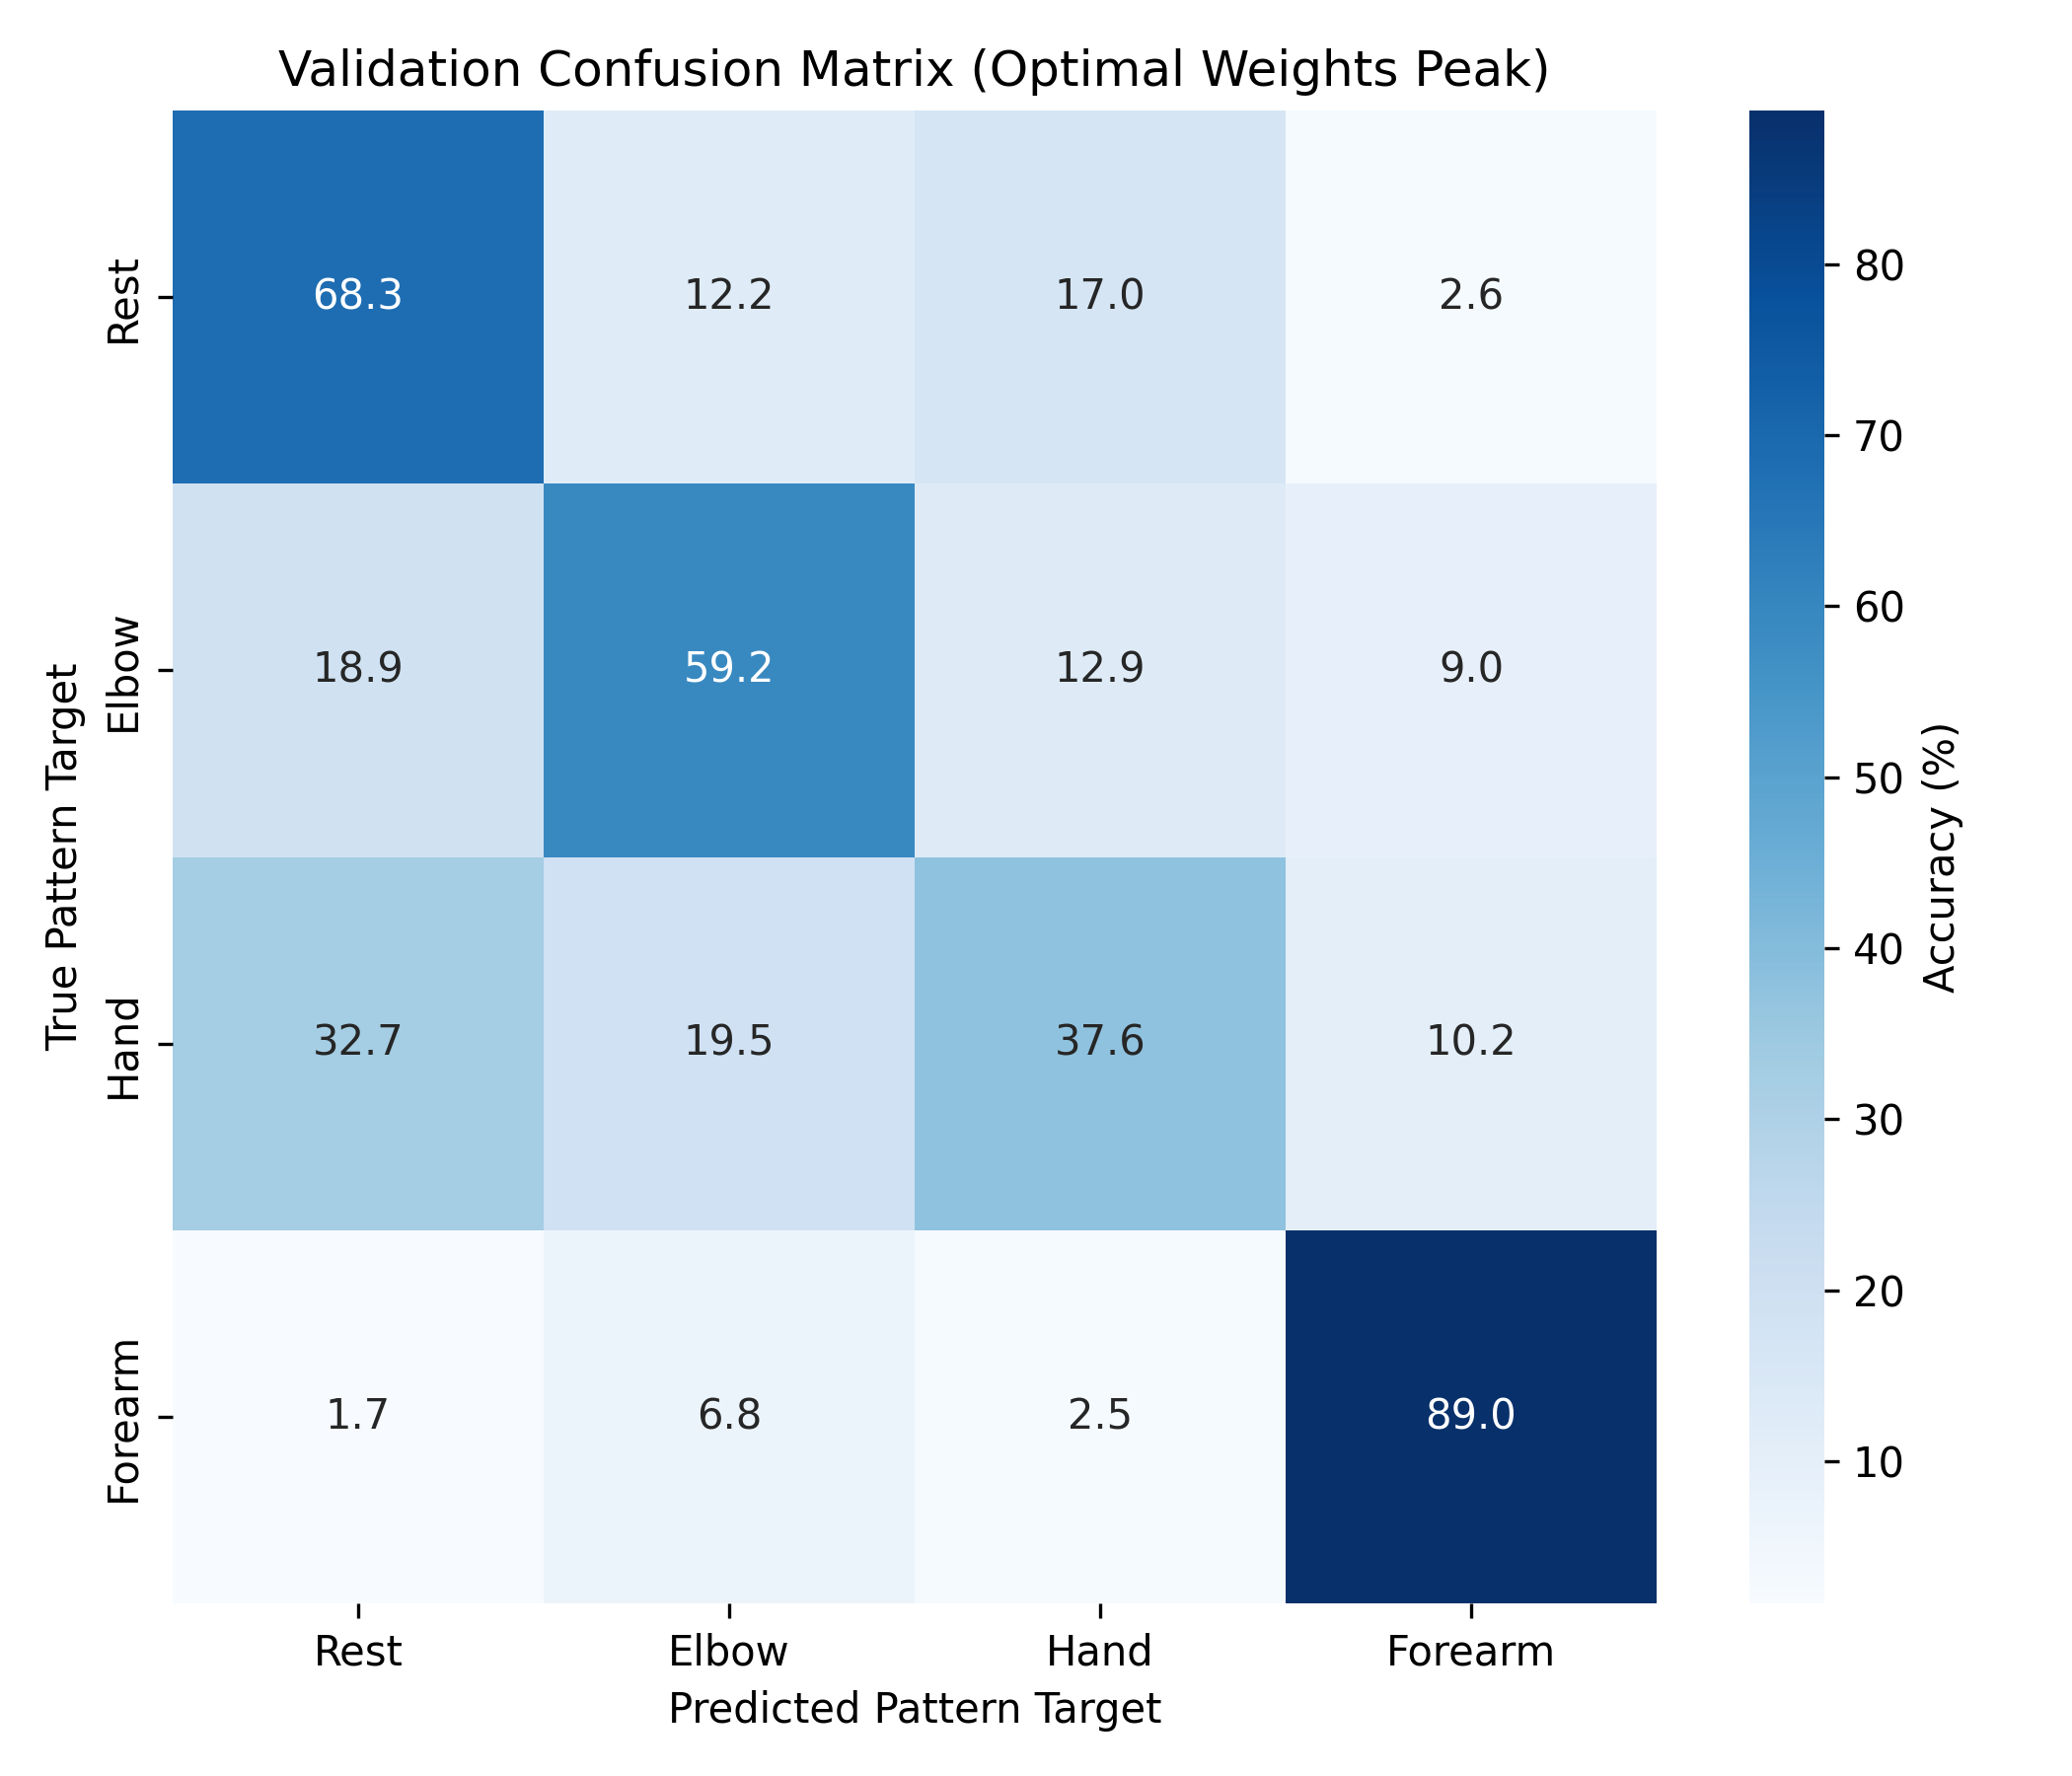
\includegraphics[width=0.324\linewidth]{models/eeg_psd/confusion_matrix.png}\hfill
  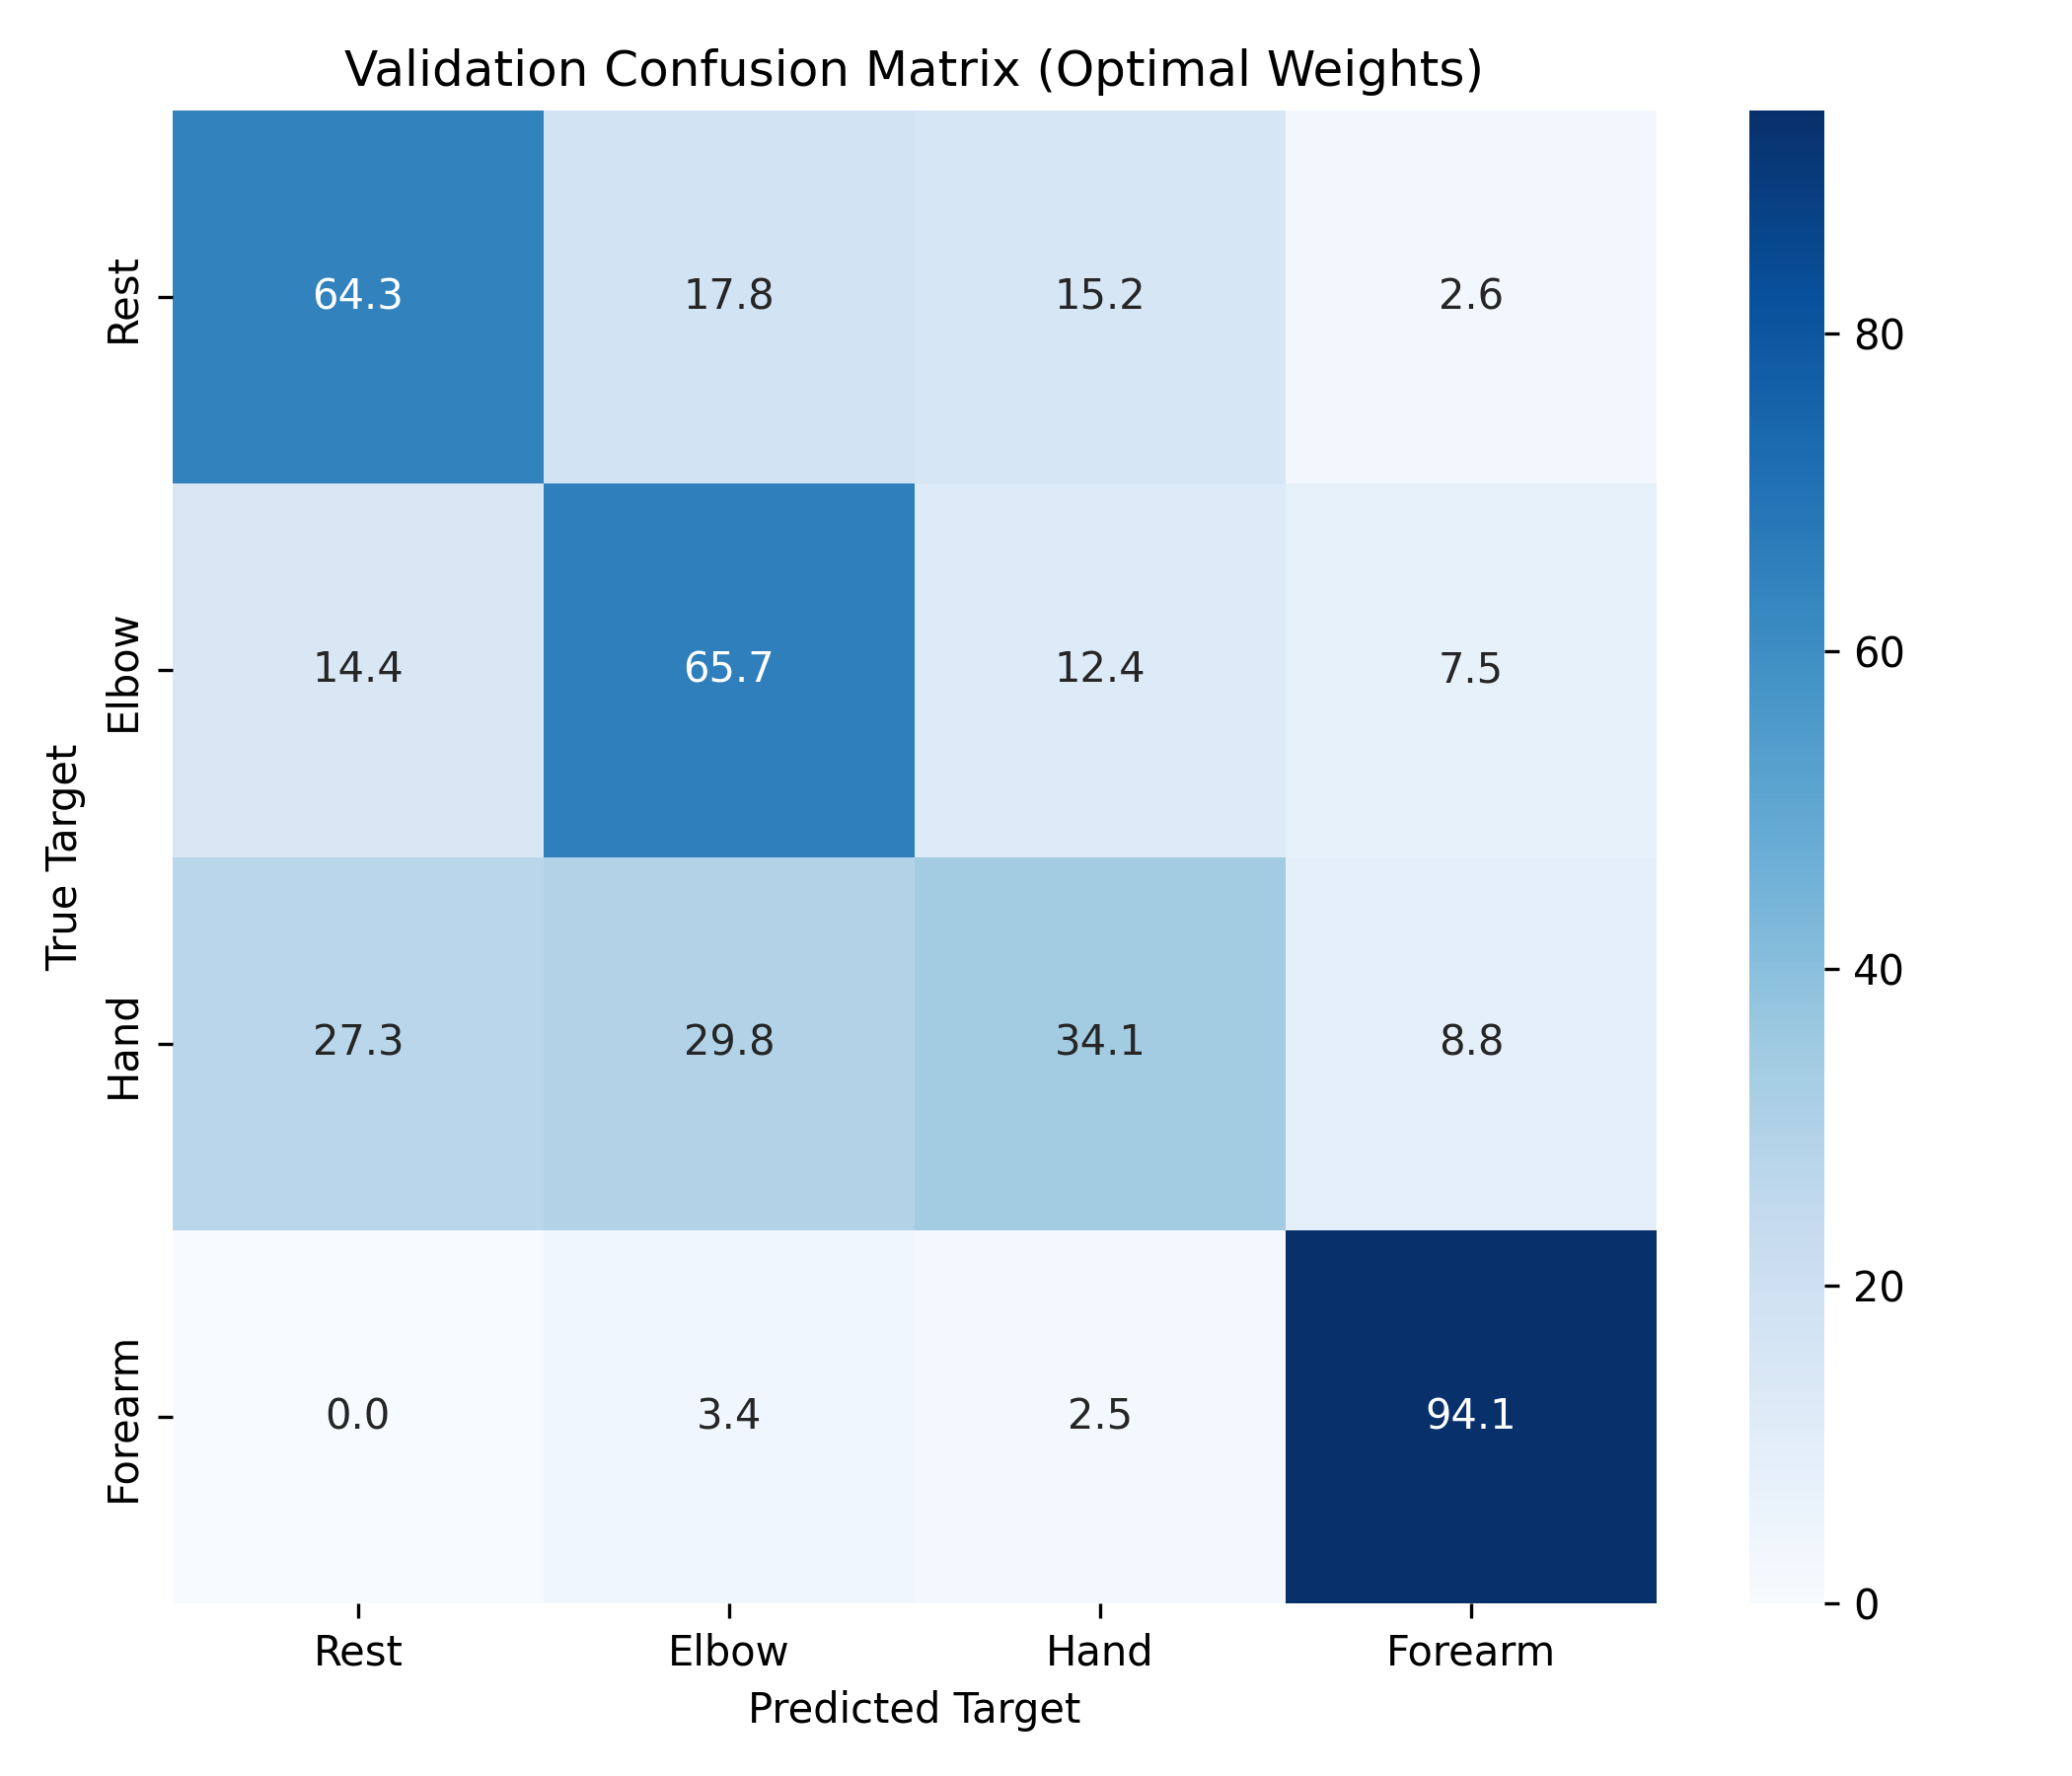
\includegraphics[width=0.324\linewidth]{models/eeg_conn/confusion_matrix.png}
  \caption{Row-normalised confusion matrices at peak validation checkpoints (percent allocated to each predicted label given a ground-truth row).}
  \label{fig:cms}
\end{figure}
